%! Author = mudtop
%! Date = 10/20/20

% Preamble
\documentclass[utf8]{report}

% Packages
\usepackage{amsmath}
\usepackage{hyperref}
\usepackage{graphicx}
\usepackage{indentfirst}
\usepackage{xcolor}
% \usepackage{classicthesis}
\usepackage[margin=.75in]{geometry}
\usepackage[T1]{fontenc}
\usepackage{newpxtext,newpxmath}
\usepackage{setspace} \doublespacing

% Ensures that all chapters start on odd pages (with intentionally blank pages on the left / even pages)
% Taken from http://mirrors.ctan.org/macros/latex/unpacked/latex.ltx
\makeatletter
\def\cleardoublepage{\clearpage\ifodd\c@page\else
    \hbox{}\newpage\if@twocolumn\hbox{}\newpage\fi\fi}
\makeatother

% Copying some formatting from Frontiers in Physics Journal 


% \newcommand{\shl}[1][0]{\emph{$shl\_mhd\_*.out$ }}
\newcommand{\mhd}[1][0]{magnetohydrodynamic }
\newcommand{\Mhd}[1][0]{Magnetohydrodynamic }
\newcommand{\BATS}[1][0]{BATS-R-US }
\newcommand{\Alfven}[1][0]{Alfv\'{e}n }
%\newcommand{\TimeDer}[1][0]{$\frac{\partial }{\partial t}$}
% Document
\begin{document}

%Start Title Page
\pagenumbering{gobble} % This command and the latter \pagenumbering{Arabic} remove the title page from the page numbering count
\vspace*{\fill}
\begin{center}
\begin{Huge}
Necronomicon
\end{Huge}

\begin{huge}
Christian-Andrew Todd Bagby-Wright
\end{huge}

\begin{normalsize}
Advisor
\end{normalsize}

\begin{Large}
Dr. Daniel Welling

Doctorate of Philosophy in Physics

University of Texas at Arlington

Arlington, Texas

United States of America

\today

\begin{normalsize}
Head of Department
\end{normalsize}

Dr. Alex Weiss

\begin{normalsize}
Examining Committee
\end{normalsize}

Dr. Amir Shahmoradi

Dr. Frederick Wilder

Dr. Yue Deng

Dr. Ramon Lopez

\end{Large}
\end{center}
\vspace*{\fill}
\newpage
%End Title Page
\pagenumbering{arabic} %Yes overleaf says that its a typo, but this is the proper command.
\tableofcontents
\listoffigures
%\listoftables
\newpage

\chapter{Introduction}
\section{Plasma Physics}

Plasma physics is defined not only by the kinetic motion of particles, but the interaction of those particles with the electric and magnetic fields. To understand the motion of plasma, we must first understand how a single test particle will move within a electromagnetic field. We must then study how many charged particles collectively affect the the electromagnetic field they are moving through, before we can understand the bulk fluid motion of a plasma.

Equations \ref{eq:Faraday} through \ref{eq:Mono} are the Maxwell equations, where \textbf{E} is the electric feild, \textbf{B} is the magnetic field, \textbf{j} is the electric current, $c$ is the speed of light in a vaccum where $c = 1 / \sqrt{\mu_{0}\epsilon_{0}}$, $\mu_{0}$ is the vacuum permeability, $\epsilon_{0}$ is the permittivity of free space, and $\rho_{q}$ is the electric charge density. 

\begin{equation}
    \nabla \times \textbf{E} = - \frac{\partial \textbf{B}}{\partial t}    
    \label{eq:Faraday}
\end{equation}

\begin{equation}
    \nabla \times \textbf{B} = \mu_{0} \textbf{j} + \frac{1}{c^{2}} \frac{\partial \textbf{E}}{\partial t} 
    \label{eq:Ampere}
\end{equation}

\begin{equation}
    \nabla \cdot \textbf{E} = \frac{\rho_{q}}{\epsilon_{0}}
    \label{eq:Gauss}
\end{equation}

\begin{equation}
    \nabla \cdot \textbf{B} = 0
    \label{eq:Mono}
\end{equation}

we assume here that the relative permittivity is unity, thus $\textbf{B} = \mu_{0} \textbf{H}$, $\textbf{D} = \epsilon_{0} \textbf{E}$, and the magnetization \textbf{M} is zero. An important consequence of Maxwell's equations is the conservation of charge which can be seen by taking the derivative of Ampere's Law and combining it with the principal of no magnetic monopole yielding: 

\begin{equation}
    \nabla \cdot (\nabla \times \textbf{B} ) = \nabla \cdot (\mu_{0} \textbf{j}) + \frac{1}{c^{2}} \frac{\partial \textbf{E}}{\partial t}
    \label{eq:ConserveCharge1}
\end{equation}

which becomes: 

\begin{equation}
    0 = \frac{\partial \rho_{q}}{\partial t} + \nabla \cdot \textbf{j}
    \label{eq:ConserveCharge}
\end{equation}

\subsection{Generalized Drift Velocity}
Maxwell's equations govern how the magnetic and electric fields behave. The particles are governed by: 

\begin{equation}
    m \frac{\partial \textbf{v}}{\partial t} = q ( \textbf{E} + \textbf{v} \times \textbf{B}) + \textbf{F}_{g} + m \frac{\partial \textbf{v}}{\partial t}\mid_{c}
    \label{eq:PP.A}
\end{equation}

where m is the particle mass, \textbf{v} is the particle velocity, $\textbf{F}_{g}$ is the force due to non-electrcomagnetic sources, and m$\frac{\partial \textbf{v}}{\partial t}|_{c}$ is the momentum change due to collisions. In most cases the last two terms of \ref{eq:PP.A} are negligible. In those cases \ref{eq:PP.A} simplifies to the Lorentz force: 

\begin{equation}
    m \frac{\partial \textbf{v}}{\partial t} = q ( \textbf{E} + \textbf{v} \times \textbf{B}) 
    \label{eq:PP.B}
\end{equation}

where it should be noted that the velocity and electric field are frame dependent. Thus to discuss the motion of a test particle through an electromagnetic field we require information about the frame. The reader should also note that the equations presented in this derivation are non-relativistic, and are thus invariant under Galilean transformations. Note that in the Lorentz force we see that only the perpendicular magnetic field affects particle motion, and that the magnetic field does not change the particle energy. 

In the case with no electric field equation \ref{eq:PP.B} becomes: 
    
\begin{equation}
    \frac{\partial \textbf{v}_{\perp}}{\partial t} = \frac{q}{m} (\textbf{v}_{\perp} \times \textbf{B}) 
    \label{eq:PP.C}
\end{equation}

whose second order derivative with respect to time becomes: 

\begin{equation}
    \frac{\partial^{2} \textbf{v}_{\perp}}{\partial^{2} t} = - \frac{q^{2}}{m^{2}} B^{2} \textbf{v}^{2}
    \label{eq:PP.D}
\end{equation}

which has the form of a harmonic oscillator with frequency $\Omega = |qB/m|$. $\Omega$ is the gyro-frequency which corresponds to the circular motion of the test particle around the magnetic field line. Equation \ref{eq:PP.D} means that a particle will tend to orbit a field line in a 2-D plane in the absence of an electric field, and any other external forces. Assuming that the positive z-axis of a right handed cordinate system is parrell to \textbf{B}, then: 

\begin{equation}
    \frac{\partial }{\partial t} v_{x} = \pm \Omega v_{y}
    \label{eq:PP.E}
\end{equation}

where the sign of $\Omega$ changes based on the sign of the test particle. If we assume, 

\begin{equation}
    v_{x} = - v_{\perp} \sin(\Omega t) 
    \label{eq:PP.F}
\end{equation}

then, 

\begin{equation}
    v_{y} = \mp v_{\perp} \cos(\Omega t) 
    \label{eq:PP.G}
\end{equation}

by integrating equations \ref{eq:PP.F} and \ref{eq:PP.G} we find that: 

\begin{equation}
    x = x_{0} + \frac{v_{\perp}}{\Omega} \cos(\Omega t)
    \label{eq:PP.H}
\end{equation}

and, 

\begin{equation}
    y = y_{0} \mp \frac{v_{\perp}}{\Omega} \sin(\Omega t)
    \label{eq:PP.I}
\end{equation}

a positively charged particle will be at x = ($x_{0} + v_{\perp}/\Omega, y_{0}$) at time t = 0 and at x = ($x_{0}, y_{0} - v_{\perp}/\Omega$) at one quarter gyro-period. Thus, a positive particle preforms a left-handed gyration, while a negative particle preforms a right-handed motion. It might be tempting at this point to attribute phenomena such as the ring current to an effect such as this. However, it is important to remember that we are discussing a test particle which does not affect the fields through which it travels. The recursive relationship between the movement of plasma and the electromagnetic fields that plasma carries is at the heart of plasma physics and something we are building to, but not yet at. Thus we should be careful about attributing large scale phenomena to the results currently being derived. The radius of gyration is $r_{L} = \rho_{g} = v_{\perp} / \Omega$, which is known as the Larmor radius. 

Now let us assume that there is a uniform electric field \textbf{E}, 

\begin{equation}
    \frac{\partial }{\partial t} \textbf{v} = \frac{q}{m} (\textbf{E} + \textbf{v} \times \textbf{B}) 
    \label{eq:PP.J}
\end{equation}

If we break equation \ref{eq:PP.F} into parallel and perpendicular (with respect to the magnetic field) components we find that for the parallel part, 

\begin{equation}
    \frac{\partial }{\partial t} \textbf{v}_{||} = \frac{q}{m} \textbf{E}_{||}
    \label{eq:PP.K}
\end{equation}

which has the rather humorous implication that the particle will reach relativistic energies very quickly in the presence of even a small electric field parallel to a magnetic field. Fortunately in reality electric fields  with such an orientation are short lived and localized. Typically this value only matters in the case of the plasma skin depth $c / \omega_{pe}$ and the plasma-wave period $2\pi / \omega_{pe}$, where $\omega_{pe}$ is the electron plasma frequency, a concept we will come back to. If then we assume that $\textbf{E}_{||} = 0$ then $\textbf{v}_{||} = 0$ and we are once agin left with only the perpendicular part of the equaiton: 

\begin{equation}
    \frac{\partial^{2} }{\partial^{2} t} \textbf{v}_{\perp} = \frac{q^{2}}{m^{2}} (\textbf{E} \times \textbf{B} - \textbf{v}_{\perp}B^{2})
    \label{eq:PP.L}
\end{equation}

assuming that $\textbf{v}_{\perp} = \Tilde{\textbf{v}} + \textbf{v}_{E}$, where $\textbf{v}_{E}$ is a constant. Then, 

\begin{equation}
    \frac{\partial^{2} }{\partial^{2} t} \Tilde{\textbf{v}}_{\perp} = - \frac{q^{2}B^{2}}{m^{2}} \Tilde{\textbf{v}}_{\perp}
    \label{eq:PP.M}
\end{equation}

and, 

\begin{equation}
    \textbf{v}_{E} = \frac{\textbf{E}\times\textbf{B}}{B^{2}}
    \label{eq:PP.N}
\end{equation}

Thus with a uniform perpendicular electric field the particle motion has two components, a gyro-motion about a magnetic field line, and a drift caused by the $\textbf{E} \times \textbf{B}$ term. This second drift is in fact known as the $\textbf{E} \times \textbf{B}$ drift, and is interestingly charge and mass independent. We also see that are assumption of $\textbf{v}_{E}$ being constant is justified. In the case of a time-stationary magnetic field there is no induction electric field and $\textbf{E} = -\nabla \phi$ where $\phi$ is the electric potential. In this case the $\textbf{E} \times \textbf{B}$ follows lines of equi-potential. Of course in the particularly of space physics there is no time-stationary magnetic field, however we will see a feature similar to this when we discuss the plasmasphere and plasmasheet. 
The $\textbf{E} \times \textbf{B}$ drift can be generalized to a velocity independent force by allowing \textbf{E} to be replaced. In fact if we recognize that \textbf{F} = q\textbf{E} and that \ref{eq:PP.N} is a specialized form of a general drift due to a velocity independent force, then we merely need to rewrite it: 

\begin{equation}
    \textbf{v}_{F} = \frac{\textbf{F}\times\textbf{B}}{qB^{2}}
    \label{eq:PP.O}
\end{equation}

\subsection{Adiabatic Invariants}

Following the method of Ruessell and Strangeway for deriving the adiabatic invariants, we begin by developing the principal of a guiding center of motion and the magnetic moment. We assume that the fields change slowly with respect to the gyro-period, or that the scale lengths are much longer then the gyro-radius, which is the definition of adiabatic. We retain the coordinate system in which the positive z-axis points along the direction of the magnetic field from above, and add the stipulation that the positive y-axis is in the direction of the electric field. Thus, $\textbf{v} = (v_{E}, 0, v_{||})$ in addition to a gyration around this drift velocity. 

If the $\textbf{E} \times \textbf{B}$ field changes very little over the gyro-radius and gyro-period then we can assume the fields are constant for the purpose of the steady state requirement in our solution to the generalized drift in eq. \ref{eq:PP.O}. In this case the motion of the particle has two parts, the fast gyro-motion around a magnetic field line, and a slow guiding center drift which does not disturb the gyro-motion. Under this adiabatic assumption we define the first adiabatic invariant to be the magnetic moment of the particle. The magnetic moment can be found by integrating Faraday's Law eq. \ref{eq:Faraday}: 

\begin{equation}
    2 \pi \rho_{g} E_{\phi} = -\pi \rho^{2}_{g} \frac{\partial }{\partial t} \textbf{B} 
    \label{eq:PP.P}
\end{equation}

where the line and surface integrals are defined by the particle gyration. Therefore, 

\begin{equation}
    m \frac{\partial }{\partial t} \Tilde{v}_{\perp} = \frac{|q|}{2} \rho_{g} \frac{\partial }{\partial t} B = \frac{m\Tilde{v}_{\perp}}{2B} \frac{\partial }{\partial t} B
    \label{eq:PP.Q}
\end{equation}

We define $W_{\perp} = 1/2 m \textbf{v}^{2}_{\perp}$ to be the perpendicular kinetic energy of the particle. By substituting this into \ref{eq:PP.Q} we find, 

\begin{equation}
    \frac{\partial }{\partial t} W_{\perp} = \frac{W_{\perp}}{B} 
    \label{eq:PP.R}
\end{equation}

The current in the loop defined by gyration is: 

\begin{equation}
    \textbf{I} = -\frac{|q|\Omega}{2\pi} \hat{\Tilde{\textbf{q}}}
    \label{eq:PP.S}
\end{equation}

where $\hat{\Tilde{q}}$ is the azimuthal direction in our cylindrical coordinate system sharing the positive z-axis with our Cartesian system. Recalling that the magnitude of the dipole moment from a  current loop is IA, where A is the area of the current loop: 

\begin{equation}
    \boldsymbol\mu = -\frac{|q|\Omega}{2\pi} \pi \frac{\Tilde{v}^{2}_{\perp}}{\Omega^{2}} \hat{\textbf{b}} = - \frac{W_{\perp}}{B} \hat{\textbf{b}}
    \label{eq:PP.T}
\end{equation}

where $\boldsymbol\mu$ is the magnetic moment. The magnetic moment was also given a vector to emphasize that it will always oppose an externally applied magnetic field, making the particles in a plasma diamagnetic. Equation \ref{eq:PP.T} demonstrates that $\boldsymbol\mu$ is invariant under a magnetic field changing slowly in time. Now we will consider a field which varies slowly spatially. An example of such a field is the narrowing of Earth's magnetic field lines as they approach to poles of Earth. The narrowing of Earth's magnetic field near the poles will give rise to a phenomena known as magnetic mirroring, a concept we will discuss in detail later, and will eventually lead us to the second adiabatic invariant. As a particle is moving along a steady state magnetic field line with spatial variations, then within the particles frame, the magnetic field is varying in time. If the particle is moving with velocity $v_{||}$ then the time varying magnetic field (in the particle's rest frame) will have the form: 

\begin{equation}
    \frac{\partial }{\partial t} B = \textbf{v}_{||} \cdot \nabla B_{z}
    \label{eq:PP.V}
\end{equation}

Thus the particles perpendicular energy would increase. However, the magnetic field is in fact steady state so there is no induction field in the stationary frame. The total energy of the particle is constant as a result, and therefore for to compensate for the perpendicular energy increasing, the parallel energy must decrease reducing $v_{||}$. Formally, due to \ref{eq:Mono}: 

\begin{equation}
    \frac{1}{\rho} \frac{\partial}{\partial t} (\rho B_{\rho}) = -\frac{\partial B}{\partial z}
    \label{eq:PP.W}
\end{equation}

where $\rho$ represents the radial component of the cylindrical coordinate system used above. Thus, 

\begin{equation}
    \delta B \approx - \frac{\rho_{g}}{2} \frac{\partial B}{\partial z} \approx - \frac{\Tilde{v}_{\perp}}{2\Omega} \frac{\partial B}{\partial z}
    \label{eq:PP.X}
\end{equation}

plugging this back into \ref{eq:PP.B} the z-component gives: 

\begin{equation}
    m \frac{\partial}{\partial t}\Tilde{v}_{||} = -|q| \Tilde{v}_{\perp} \delta B = -\mu \frac{\partial}{\partial z} B
    \label{eq:PP.Y}
\end{equation}

after substituting the approximation from \ref{eq:PP.X}. For the azimuthal component we find that: 

\begin{equation}
    m \frac{\partial}{\partial t}\Tilde{v}_{\perp} = |q| v_{||} B_{\rho} = \frac{|q|\Tilde{v}_{\perp} v_{||}}{2\Omega} \frac{\partial}{\partial z} B = \mu \frac{v_{||}}{\Tilde{v}_{\perp}} \frac{\partial}{\partial z} B
    \label{eq:PP.Z}
\end{equation}

Equation \ref{eq:PP.Z} is sign independent in relation to the charge, however that is a result of the notation used. Positively (negativity) charged particles will gyrate in a left-handed (right-handed) way. By combining \ref{eq:PP.Y} and \ref{eq:PP.Z} we note that $d(W_{||} + W{\perp} / dt) = 0$, a statement of the conservation of energy, which while unsurprising is reassuring to derive as a byproduct of the adiabatic invariance of the magnetic moment which is nearly complete. By rearranging terms in \ref{eq:PP.Z} we find that: 

\begin{equation}
    \frac{d W_{\perp}}{dt} = \mu v_{||} \frac{\partial B}{\partial z}  = \mu \frac{\partial B}{\partial t} \therefore \frac{d \mu B}{dt} = \mu \frac{dB}{dt} 
    \label{eq:PP.AA}
\end{equation}

hence, 

\begin{equation}
    \frac{d\mu}{dt} = 0
    \label{eq:PP.BA}
\end{equation}

Thus, the magnetic moment is constant under both slow temporal and spatial changes, closing our derivation of the magnetic moments adiabatic invariance. The invariance of the magnetic moment leads to a phenomena called betatron acceleration, in which if the magnetic field increases slowly with time then the perpendicular energy of the particle will also increase. 

The second adiabatic invariant is the name of the other invariant value associated with a slow changing field, such as those caused by Earth's pole. It is defined as: 

\begin{equation}
    J = \oint p_{||} ds
    \label{eq:PP.CA}
\end{equation}

where the integral is taken along the path of the guiding center motion, with the integral being done between the mirror points, and $p_{||}$ is the parallel momentum. Since, 

\begin{equation}
    \frac{p^{2}_{||}}{2m} = W - \mu B = \mu (B_{m} - B) 
    \label{eq:PP.DA} 
\end{equation}

where $B_{m}$ is the magnetic field at the mirror point. Thus, 

\begin{equation}
    J = \sqrt{2m\mu} \oint (B_{m} - B)^{1/2} ds 
    \label{eq:PP.EA}
\end{equation}

Therefore if the magnetic field changes slowly with respect to the surface over which the integration is taken then $B_{m} - B$ is effectively zero. This demonstrates that under an adiabatic condition $J$ is an adiabatic invariant. Similar to the magnetic moment, when the second adiabatic invariant is in fact, variant, an acceleration is caused to act on the particle known as Fermi acceleration. Fermi acceleration occurs when two magnetic mirror points move closer together, as can happen with mirror points in the solar wind and the bow shock. 

\subsection{Kinetic Theory} 

In the previous sections we have shown how a single test particle will move through an electromagnetic field. From this simplified approach we have already seen some important concepts of plasma physics such as the conservation of mass, charge, energy, and the adiabatic invariants. With this basic understanding we can begin to build up a proper theory of how a plasma will behave when the fields are allowed to change in time. This recursive relationship between many moving charged particles and time varying electromagnetic fields is best resolved through a statistical approach. Let us define a distribution function $f$, as a function of position in three space, velocity, and time, $f(\textbf{r}, \textbf{v}, t)$, where $\textbf{r}$ is the position vector and $\textbf{v}$ is the velocity vector. Let us also define the acceleration of the particles as $\textbf{a} \equiv d\textbf{v}/dt$. The term phase space density can also be used to describe the distribution function. We can then write a conservation equation for this value: 

\begin{equation}
    \frac{\partial}{\partial t} f + \frac{\partial}{\partial \textbf{r}} \cdot (f\textbf{v}) + \frac{\partial}{\partial \textbf{v}} \cdot (f\textbf{a}) = \frac{\partial}{\partial t} f\vert_{c}
    \label{eq:KT.1}
\end{equation}

In this notation \textbf{v} is independent of the position, as it is a separate set of coordinates in the phase space.  The term on the right hand side includes all collisional forces including friction. Thus, on the left hand side of the equation the acceleration of the particles is also independent of the velocity except for the \textbf{v} $\times$ \textbf{B} force (the portion of the acceleration caused by friction being separated out and merged into the term on the right-hand side). Because \textbf{v} $\times$ \textbf{B} is perpendicular to \textbf{v}, $\nabla_{\textbf{v}} \cdot (\textbf{v} \times \textbf{B}) =0$, where we introduce the notation, $\nabla_{\textbf{v}} = \partial / \partial \textbf{v}$. As a result we can rewrite \ref{eq:KT.1} as: 

\begin{equation}
    \frac{\partial}{\partial t} f + \textbf{v} \cdot \nabla f + \textbf{a} \cdot \nabla_{\textbf{v}} f = \frac{\partial}{\partial t} f|_{c}
    \label{eq:KT.2}
\end{equation}

This is the Boltzmann equation. If collisions are considered to be negligible then \ref{eq:KT.2} becomes the Vlasov equation: 

\begin{equation}
    \frac{\partial}{\partial t} f + \textbf{v} \cdot \nabla f + \textbf{a} \cdot \nabla_{\textbf{v}} f = 0
    \label{eq:KT.3}
\end{equation}

This does assume that in the absence of collisions, the phase space density is a conserved quantity. We can simplify the notation by defining the Liouville operator $\mathcal{L} = \partial / \partial t + \textbf{v} \cdot \nabla + \textbf{a} \cdot \nabla_{\textbf{v}}$. The Liouville operator is the gradient along the particle's trajectory as $\textbf{a} \equiv d\textbf{v}/dt$ and $\textbf{v}=d\textbf{r}/dt$. This has the consequence that the phase space density along a particle's trajectory is constant. By assuming that a particle at position \textbf{r}, and velocity \textbf{v}, at some time t, moves to \textbf{r}', \textbf{v}', at some latter time t', and placing both of these into \ref{eq:KT.3} we find that,  $f(\textbf{r}, \textbf{v}, t) = f(\textbf{r}', \textbf{v}', t')$. , This is known as Liouville's theorem.

By using the Boltzmann equation and the Liouville theorem we can derive several important aspects of plasma physics. By allowing the distribution function to be a maxwellian velocity distribution, 

\begin{equation}
    f = \frac{n}{(2\pi KT)^{1/2}}\exp(\frac{-v^{2}}{2mKT})
    \label{eq:KT.4}
\end{equation}

where $n$ is the density of the plasma, and $m$ is the species mass, $T$ is the temperature and $K$ is the Boltzmann constant. 
By using this form of a distribution function, we can make use of Maxwell's equations with reasonable boundary conditions, such as the electric potential going to zero at infinity, to derive several key properties of a plasma, namely the electron plasma frequency, 

\begin{equation}
    w^{2}_{pe} = \frac{n_{e} e^{2}}{\epsilon_{0} m_{e}}
    \label{eq:KT.5}
\end{equation}

where $w_{pe}$ is the electron plasma frequency, $n_{e}$ is the electron density, $e$ is the electron charge, $m_{e}$ is the mass of the electron, and $\epsilon_{0}$ is the permittivity of free space. We can also use the \ref{eq:KT.4} to derive the Debye length. The Debye length is the characteristic length over which an isolated charge in a plasma is shielded form the plasma. In the previous section discussing the adiabatic invariants we stated that the conditions had to change slowly over both time and space. The gyro-period was the characteristic time which had to be respected, and the Debye length is the characteristic length over which the electromagnetic fields could only vary slowly. The Debye length is, 

\begin{equation}
    \lambda_{D} = (\frac{\epsilon_{0} KT}{n e^{2}})^{1/2}
    \label{eq:KT.6}
\end{equation}

where $\lambda_{D}$ is the Debye length. Another parameter related to the Debye length is the number of particles in the Debye sphere, a sphere whose radius is the Debye length, known as the Debye number

\begin{equation}
    N_{D} = \frac{4}{3} \pi n \lambda^{3}_{D}
    \label{eq:KT.7}
\end{equation}

Within a plasma a charged particle only experiences electromagnetic effects from particles within its Debye sphere, beyond that the particle is shielded by the roughly even distribution of protons and electrons in the plasma. When the scale length of a system is large compared to the Debye length it is said to be quasinuetral. Quasineutrallity is so important to the behavior of plasmas that the space plasma physics textbook \cite{Rycroft1998BasicSP} %I literately used \cite's own search function to get the key. Why doesn't it recognize it?
includes quasineutrallity in its definition of a plasma. Both \ref{eq:KT.6} and \ref{eq:KT.7} assume that the ion and electron temperatures are similar. If they are not then the characteristic length of the plasma can be found as, 

\begin{equation}
    \frac{1}{\lambda^{2}} = \frac{1}{\lambda^{2}_{De}} + \frac{1}{\lambda^{2}_{Di}}
    \label{eq:KT.8}
\end{equation}
    


From this the Debye sphere and Debye number can be recalculated using the appropriate Debye length. 

In summary, a kinetic approach to plasma physics allows us to improve the single-orbit theory by adding in the effects of many different particles on each other and on the electromagnetic field through which they traverse. However, it is not practical to calculate the Vlasov equation for each particle in a plasma. Even in the vacuum of space, densities of plasma can reach several thousands of particles per cubic centimeter. As such, in the next section the theory of magnetohydrodynamics will be introduced, and its basic principles and equations derived. 

\subsection{Magnetohydrodynamics}

Magnetohydrodynamics (MHD) takes a fluid approach to plasma physics. As the name implies it takes hydrodynamics, the study of fluid flow, and adds electromagnetism on top of it. Why it isn't called electromagnetohydrodynamics is a mystery left to an English major. In the case of MHD we take the Boltzmann equation from the kinetic approach and use it to find and calculate the evolution of the bulk properties of a plasma directly. A key assumption in MHD is that the plasma is localized, meaning that at a point of measurement the forces, particles, or fields causing a change in parameters at that measurement point are near the point themselves. It is difficult to prove the true locality of a plasma in space practically speaking. The Louiville theorem implies that a plasma should have significant structure to it. As particles from a hot portion of the phase space density enter the same region as particles from a c old part of the phase space there are no collisions (as a result of our assumption of a collisionless plasma) to mix the plasma, and thus the phase space density. It is assumed that local processes, not gone into detail here, will mix the phase space densities of the hot and cold plasmas. This is what is meant by a localized plasma. 

To derive the continuity, momentum, and energy equations we first derive a general form. Taking a moment integral of the Boltzmann equation over the velocity space of the phase space density, 

\begin{equation}
    \int \varphi(\textbf{v}) \frac{\partial}{\partial t} f d^{3}v + \int \varphi(\textbf{v})\textbf{v} \cdot \nabla f d^{3}v + \int \varphi(\textbf{v})\textbf{a} \cdot \nabla_{\textbf{v}} f d^{3}v 
    = \int \varphi(\textbf{v})\frac{\partial}{\partial t}f |_{c} d^{3}v 
    \label{eq:MHD.1}
\end{equation}

Where $\varphi(\textbf{v})$ is an unspecified function of \textbf{v}. Once we have found a general solution for $\varphi(\textbf{v})$ we can substitute in equations for the density, momentum, energy, etc. By rewriting some of the integrals in terms of their expectation values, and limiting the distrobution $f$ such at  $\varphi(\textbf{v})f \rightarrow 0$ at infinity faster then $\textbf{v} \rightarrow \infty$, we arrive at, 

\begin{equation}
    \frac{\partial}{\partial t} (n\langle\varphi(\textbf{v})\rangle) + \nabla \cdot (n\langle\textbf{v}\varphi(\textbf{v})\rangle) - n\langle(\textbf{a}\cdot\nabla_{\textbf{v}})\varphi(\textbf{v})\rangle = \frac{\partial}{\partial t} (n\langle\varphi(\textbf{v})\rangle)|_{c}
    \label{eq:MHD.2}
\end{equation}

where we have still not defined the collisionial term on the right hand side of the equation. Equation \ref{eq:MHD.2} is the generalized form of the MHD equations. To get a specific MHD equation, such as the momentum equation, we substitute $\varphi(\textbf{v})$ for a specific form. Something to note is that the time rate of change of our unspecified function, $\partial \varphi(\textbf{v}) / \partial t$ is depended on the a divergence, $\nabla \cdot \langle \textbf{v} \varphi(\textbf{v}) \rangle$. Therefore as a solution to the equation requires knowledge of a higher order solution we must make assumptions to close the system of equations. The fluid description of MHD is altered for each species in the plasma, however for their presentation here I will show single-fluid MHD, in which the species will be summed over to arrive at a single equation describing the entire plasma. In this case, the pressure is defined in relation to the plasma bulk flow, as opposed to the flow of the individual species within the plasma. 

For the zero-order moment we define $\varphi(\textbf{v}) = 1$. Plugging this into \ref{eq:MHD.2}% why isn't this reference working!
and simplifying we find, 

\begin{equation}
    \frac{\partial}{\partial t} \rho + \nabla \cdot (\rho \textbf{u}) = 0
    \label{eq:MHD.3}
\end{equation}

Were we have assumed a collisionless plasma. Equation \ref{eq:MHD.3} is known as the continuity equation. We can also get the charge density equation by multiplying \ref{eq:MHD.2} by the charge q first and following the same steps as we did for \ref{eq:MHD.3}, 

\begin{equation}
    \frac{\partial}{\partial t} \rho_{q} + \nabla \cdot \textbf{j} = 0
    \label{eq:MHD.4}
\end{equation}

which is a statement of charge conservation. 

For the first order equation we specify $\varphi(\textbf{v}) = m\textbf{v}$, where $m$ is the particle species mass. Thus ref{eq:MHD.2} becomes, 

\begin{equation}
    \rho \frac{D}{Dt} \textbf{u} + \nabla \cdot \textbf{P} - \textbf{j} \times \textbf{B} = 0
    \label{eq:MHD.5}
\end{equation}

$\rho = \sum_{s} n_{s}m_{s}$, is the mass density of the plasma, $D/Dt \equiv \partial / \partial t + \textbf{u} \cdot \nabla$, \textbf{u} is the flow velocity of the plasma, $\textbf{P}$ is the pressure tensor defined as $mn\langle w_{j}w_{i} \rangle = P_{ji}$, where $\textbf{w} = \textbf{v} - \Bar{\textbf{u}}$ is the peculiar velocity, or the velocity of a species with respect to the bulk flow velocity of the plasma, and $\textbf{j} = \sum_{s} n_{s}q_{s}\textbf{u}_{s}$ is the current density. 

Finally the second order solution which is the energy equation, which can be found by allowing $\varphi(\textbf{v}) = 1/2 m v^{2}$ we can find the energy equation, 

\begin{equation}
    \frac{D}{Dt} (P\rho^{-\gamma}) = 0
    \label{eq:MHD.6}
\end{equation}

where $\gamma = (N+2)/N$ is the ratio of specific heats, and N is the degrees of freedom in the system. In the derivation of the above solutions the assumptions of quasi-neutrality, isotropic pressure, and that Joule dissipation and heat flux can be ignored were all employed. This is known as ideal MHD. 


\subsection{Frozen in Flux Theorem}  

Cold plasma particles in a collisionless plasma are bound to a specific field line which they cannot leave unless collective effects violate the adiabatic invariants. Even in energetic particles it takes strong effects from magnetic field gradients or curvature to disrupt the gyrating motion of the particles about their magnetic field line. Because cold plasma cannot leave the field line when external forces cause that field line to move so must the plasma move. For that same reason when the cold plasma moves, it must carry the magnetic field lines flowing through it along with its motion. As such the movement of the cold plasma and the magnetic flux tubes in it are closely related.

\begin{equation}
    \textbf{j} = \sigma_{0}(\textbf{E}+\textbf{v}\times\textbf{B})
    \label{eq:PP.1}
\end{equation}

where $\textbf{j}$ is the current, \textbf{E} is the electric field, \textbf{v} is the plasma velocity, and \textbf{B} is the magnetic field. 

Eq. \ref{eq:PP.1} is the generalized Ohm's Law valid for fully ionized geophysical plasmas where the typical collision frequencies are extremely low and the plasma conductivity can be taken as near-infinite. In eq. \ref{eq:PP.1} the resistivity was replaced by its inverse, the plasma conductivity: 

\begin{equation}
    \sigma_{0} = \frac{n_{e}e^{2}}{m_{e} \nu_{c}}
    \label{eq:PP.2}
\end{equation}

where $n_{e}$ is the electron density, $e$ is the charge of an electron, $m_{e}$ is the mass of an electron, and $\nu_{c}$ is the frequency of collisions. 

Recall Faraday's Law: 

\begin{equation}
    \nabla\times\textbf{E} = - \frac{\partial\textbf{B}}{\partial t}
    \label{eq:PP.3}
\end{equation}

where t is time. We can used the generalized Ohm's law to eliminate the electric field in Faraday's law yeilding:

\begin{equation}
    \frac{\partial\textbf{B}}{\partial t} = \nabla \times (\textbf{v}\times\textbf{B}-\textbf{j}/\sigma_{0})
    \label{eq:PP.4}
\end{equation}

Using Ampr\`{e}re's law

\begin{equation}
    \nabla\times\textbf{B} = \mu_{0}\textbf{j} + \epsilon_{0}\mu_{0}\frac{\partial \textbf{E}}{\partial t}
\end{equation}

where $\epsilon_{0}$ and $\mu_{0}$  are the vacuum permittivity and susceptibility, respectively. 

Assuming a steady state electric field and noting that $\nabla\cdot\textbf{B} = 0$, we get a general induction equation for the magnetic field:

\begin{equation}
    \frac{\partial \textbf{B}}{\partial t} = \nabla \times (\textbf{v}\times\textbf{B}) + \frac{1}{\mu_{0}\sigma_{0}}\nabla^{2}\textbf{B}
    \label{eq:PP.5}
\end{equation}

In the first term of the right hand side of the equation we see that the motion of the plasma causes the local magnetic field to change, while in the second term we see the affect of diffusion. 

By setting the velocity to be zero we kill the first term on the right hand side of equation \ref{eq:PP.5} we see the diffusion equation for the magnetic field: 

\begin{equation}
    \frac{\partial \textbf{B}}{\partial t} = D_{m}\nabla^{2}\textbf{B}
    \label{eq:PP.6}
\end{equation}

where $D_{m}$ is the diffusion coefficient defined as $D_{m} = (\mu_{0}\sigma_{0})^{-1}$.

With a finite resistance in the plasma the magnetic field tends to diffuse across the plasma and to smooth out any local inhomogeneities. In cases where this diffusion is negligible however we enter the domain of frozen-in magnetic flux. In a collisionless plasma with infinite conductivity \ref{eq:PP.5} reduces to: 

\begin{equation}
    \frac{\partial \textbf{B}}{\partial t} = \nabla \times (\textbf{v}\times\textbf{B})
    \label{eq:PP.7}
\end{equation}

Eq. \ref{eq:PP.7} implies that any field change are such that the magnetic field lines are constrained to move with the plasma. With the basics of the plasma physics important to this work established let us now move into the specifics of space environment. 

\section{Solar Wind}

% Should I include a discussion on the history of the science for each portion? i.e. when was the plasmasphere / ring current first proposed, early significant finds etc.? Or do I only cover them in the modern conception? Yes, include history. Give history and define every term. Every term. Like each one. 

The near Earth space environment is a strongly driven system. Before we can understand the dynamics of this system we must begin with understanding its driving force, the solar wind. The magnetic fields at the surface of the sun are complicated. As various magnetic systems interact plasma can be ejected from the sun through funnels, coronal holes, coronal mass ejections and other mechanisms. %Plasma will detach from the sun at the \Alfven critical point. %True but needs more of an explanation. 

Plasma moves towards Earth as part of the solar wind governed by the \mhd equations. Specific recurring geometries are created by the interactions of various flows of plasma as they balance pressure, momentum, and the geometries of their magnetic fields. The MHD equations contain information of the bulk flow velocity, collisions transfers, and sources and sinks of plasma moments. 
The variable nature of the solar wind causes asymmetries in the flow of plasma in the interplanetary magnetic field. Factors such as the co-rotation of the sun's magnetic field, sunspots, f10.7 radiation, and others contribute to the irregular flow of the solar wind.

There are several geometries of the solar wind important to my research. When these geometries reach Earth, they interact with Earth's magnetic fields in different ways, affecting the local flow of plasma. The first of these geometries is a Co-rotating Interaction Region (CIR) event, in which fast streams of the solar wind catch up to slow streams in the rotating field creating a CIR. CIRs are typically a weak kind of storm featuring an oscillating $B_{z}$ with a long recovery phase, normally on the order of several weeks. Coronal mass ejection events have two sub categories, magnetic clouds, and sheath driven. The magnetic geometry of sheath driven CME events is similar to that of CIR storms, however the two classes of storm vary in average storm length, recovery, and intensity. Magnetic Cloud type CMEs have a strong magnetic field rotated through a large angle. %(Klein and Burlaga,1982 [reference taken from Katus 2014, don't have access to it myself.)

%The remainder of this section just falls off a cliff. 
The solar wind is comprised primarily of protons, electrons, ~4\% alpha particles, and minor amounts of heavier ions. 

Due to the low density and high temperature of the solar wind kinetic effects are more important in the solar wind then in other plasma populations. Kinetic effects include things like Coulomb collisions and wave particle interactions. 

\section{Magnetosphere}

Magnetic interaction with the magnetosphere is the primary driver of dynamics near Earth. Day and Night side re connection is the dominate way in which the solar wind interacts with the magnetosphere. [\color{red}Write out a nice long explanation of the Dungey Cycle and night side re connection.\color{black}]

Other interaction regions, such as the bow shock, viscous interactions along the flank, field aligned currents. Each of these will need an explanation, gives good segue into other parts of the space environment. 
\subsection{Magnetic Storms and Reconnection}

Place Holder.

\section{Inner Magnetosphere}

The Inner Magnetosphere exists. People talk about because of all the way more interesting sub components like the...


\subsection{Plasmasphere}

%omposition, typical values of density and energy, filling / refilling rates and mechanics etc. 

%Specific discussion of important features: 
%    \begin{itemize}
%        \item dusk bulge
%        \item day side plume 
%        \item seperatrix 
%        \item borovsky's proposed 7 step process. \color{red}Should Borovsky's paper get its own section at the 
%end? Could use it to lead into science questions. If so do we repeat the process here or save it for %later.\color{black}
%    \end{itemize}
 
 The Bow shock requires a potential difference, this creates a dawn-dusk electric field (or maybe its the other way around). Combine this with the constant rotation of the magnetosphere as Earth rotates and this gives rise to another electric field pointed radially inwards towards Earth. The balance of these two fields gives rise to line of equipotential electric energy. Within the line of zero equipotential electric energy are closed drift paths, the plasmasphere.

The interaction between the solar wind and the magnetosphere creates a Dawn-Dusk electric field that exists everywhere within the magnetosphere. The interaction of the Dawn-Dusk electric field and the electric field caused by Earth's co-rotating magnetic field creates lines of equipotential within the magnetosphere. Particles within the magnetosphere will drift along these equipotential lines eventually reaching the magnetopuase and mixing with the solar wind in a viscous interaction, this is called an open drift path. Within the line of zero potential the drift paths of plasma are closed. This region is defined to be the plasmasphere.

Russel \& Strangeway states that a particle drift velocity can be generalized to any velocity-independent force $\textbf{F}$:

\begin{equation}
    \textbf{v}_{d} = \frac{\textbf{F}\times\textbf{B}}{qB^{2}}
    \label{eq:PS.1}
\end{equation}

where q is the particle charge. 

If the force can be expressed in terms of a potential, such as the electric potential for a static electric field $\textbf{F} = -q\nabla\Tilde{\phi}$, then we can rewrite the drift velocity as: 

\begin{equation}
    \textbf{v}_{d} = \frac{\textbf{B}\times\nabla\Tilde{\phi}}{B^{2}}
    \label{eq:PS.2}
\end{equation}

As a consequence, drift paths follow equipotential contours for this generalized potential. 

To explore this in more detail, with out unnecessary complexity, we will make a few simplifying assumptions. First, that Earth's magnetic field can be well represented as a magnetic dipole. Second, that Earth's magnetic dipole points along Earth's axis of rotation. Finally, that Earth's axis of rotation is perpendicular to the ecliptic plane. We shall define a coordinate system such that the positive x-axis points from the center of Earth to the center of the sun. The positive z-axis points along the dipole axis, and the y-axis completes the right-handed coordinate system. In our case this means that the positive y-axis is pointing from the center of Earth opposite the direction Earth orbits around the sun. We also define a corresponding spherical coordinate system were the azimuthal angle ($\varphi$) varies around the z-axis of the Cartesian coordinate system, with $\varphi = 0$ pointing to the sun and $\varphi = \pi / 2$ pointing along the y-axis. 

Further restricting our discussion to $90^{\circ}$ pitch angle particles drifting in the equatorial plane, and assuming steady state electric and magnetic fields, we can write the particle drift velocity as 

\begin{equation}
    \textbf{v}_{d} = \frac{-\nabla\phi \times \textbf{B}}{B^{2}} + \frac{W_{\perp}}{qB^{3}}\textbf{B} \times \nabla B
    \label{eq:PS.3}
\end{equation}

where $\phi$ is the electric field potential ($\textbf{E} = -\nabla\phi$) and $W_{\perp}$ is the perpendicular energy of the particle. Recall that a particle's magnetic moment is $\mu = W_{\perp}/B$. Therefore we can rewrite \ref{eq:PS.3} as:

\begin{equation}
    \textbf{v}_{d} = \frac{1}{B^{2}}\textbf{B} \times \nabla ( \phi + \frac{\mu B}{q} )
    \label{eq:PS.4}
\end{equation}

We can define 

\begin{equation}
    \Tilde{\phi} = \phi + \frac{\mu B}{q} = \phi + W_{\perp}
    \label{eq:PS.5}
\end{equation}

The potential that the $90^{\circ}$ equatorial particle drift paths follow. This parameter is the total energy of the particles, save for the portion of energy associated with the drift itself. 

We understand now what roll the potential plays in determining the particle drift, but what form does this potential take? Within the magnetosphere there are two primary means by which an electric potential is imposed. The first of these is corotation. Collision of neutral atoms in the atmosphere forces the ionosphere to corotate, creating a corotation electric field. In the steady state magnetic field lines are equipotentials, causing the electric potential in the ionosphere to map down to the equatorial plane. However this is where our assumptions breakdown somewhat. In actuality the changes in convection are transmitted through magnetohydrodynamic waves and the associated Maxwell stress ($\textbf{j} \times \textbf{B}$). The other source of the electric potential is the convection from the night side to the day side of the planet. This convection is driven by reconnection with the IMF, and sun ward convection returns magnetic flux that is in turn transported into the lobes vie the reconnection process. 

For corotation, 

\begin{equation}
    \textbf{v}_{cr} = \hat{\boldsymbol{\varphi}} r \frac{2\pi}{\tau_{d}}
    \label{eq:PS.6}
\end{equation}

where $\tau_{d} = 86,400$ is the number of seconds in the day. Working backwards from this we see that the corresponding electric potential is: 

\begin{equation}
    \phi_{cr} = -\frac{2\pi}{\tau_{d}}B_{0}r_{0}^{2}(\frac{r_{0}}{r})
    \label{eq:PS.7}
\end{equation}

In equation \ref{eq:PS.6} we have retained our assumption of a dipole magnetic field described as $B = B_{0}r_{0}^{3}/r^{3}$. Referencing the International Geomagnetic Reference Field (IGRF) to specify the dipole magnetic field, the $r_{0}$ is the mean Earth radius (6371.2 km). 

We can further define a parameter known as the corotation potential: 

\begin{equation}
    \phi_{c} = \frac{2\pi}{\tau_{d}}B_{0}r^{2}_{0}
    \label{eq:PS.8}
\end{equation}

Using the IGRF version 12 magnetic field for 2016, $B_{0} = 29816$ nT and $\phi_{c} = 88.01 kV$. 

For the reconnection-imposed convection we make the simplifying assumption that the electric field is uniform and points from dawn to dusk (positive-y direction): 

\begin{equation}
    \textbf{E}_{conv} = \hat{\textbf{y}} \frac{\phi_{pc}}{Wr_{0}}
    \label{eq:PS.9}
\end{equation}

where $\phi_{pc}$ is the cross-polar-cap potential and W is a characteristic width of the magnetosphere, expressed in units of $r_{0}$. There are more sophisticated models of the convection electric field, for example the Volland-Stern model, where the convection electric field is shielded from the inner magnetosphere. But for the purpose of understanding how the plasmasphere arises from the interaction of the electric fields, the uniform electric field assumption is sufficient. 

Now let us derive the potential corresponding to the electric field in \ref{eq:PS.8} Combining this with the corotation potential, we get the total potential for the sunward convection and corotation: 

\begin{equation}
    \phi = -\phi_{c} (\frac{r_{0}}{r}) - \frac{\phi_{pc}}{W}(\frac{r}{r_{0}})\sin{\phi}
    \label{eq:PS.10}
\end{equation}

At any particular radial distance the potential is maximum at dawn $(\phi = -\pi/2)$ and minimum at dusk $(\phi = \pi/2)$. The potential lies between these two limits for any other local times. 

For equatorial particles, then, from eq \ref{eq:PS.5}, 

\begin{equation}
    \Tilde{\phi} = -\phi_{c} (\frac{r_{0}}{r}) - \frac{\phi_{pc}}{W}(\frac{r}{r_{0}})\sin{\phi}+\frac{\mu B_{0}}{q} (\frac{r_{0}}{r})^{3}
    \label{eq:PS.11}
\end{equation}

or

\begin{equation}
    \frac{\Tilde{\phi}}{\phi_{c}} = -(\frac{B}{B+{0}})^{\frac{1}{3}} - \frac{\phi_{pc}}{W\phi_{c}}(\frac{B_{0}}{B})^{\frac{1}{3}}\sin{\phi} + \frac{\mu B_{0}}{q\phi_{c}}(\frac{B}{B_{0}})
    \label{eq:PS.12}
\end{equation}

in eq \ref{eq:PS.11} the magnetic moment is normalized to $\mu = q \phi_{pc} / B_{0}$. In SI units this parameter equals 2.948 $GeVT^{-1}$. By combining equations \ref{eq:PS.2} and \ref{eq:PS.10} the equatorial particle drift velocity is given by

\begin{equation}
    \textbf{v}_{d} = \frac{2\pi r_{0}}{\tau_{d}} \{ \hat{{\varphi}} [(\frac{r}{r_{0}}) - \frac{\phi_{pc}}{W\phi_{c}}(\frac{r}{r_{0}})^{3}\sin{\phi} - \frac{\mu B_{0}}{q\phi_{c}}(\frac{r_{0}}{r})]+\hat{\boldsymbol{r}}\frac{\phi_{pc}}{W\phi_{c}}(\frac{r}{r_{0}})^{3}\cos{\phi}\}
    \label{eq:PS.13}
\end{equation}

If we consider the azimuthal component of eq. \ref{eq:PS.13}, the first term in the square brackets corresponds to corotation and the second corresponds to the $\varphi-$component of the sunward convection. The last term in the square brackets is the gradient drift. Note that the gradient drift of positive ions of the plasma is counter to the drift of corotation. Eq. \ref{eq:PS.13} shows that the different drifts tend to dominate at different radial distances. At small radial distances, the gradient drift will tend to dominate; at large radial distances, sunward convection dominates; at intermediate distances, corotation is important. But, again, this is complicated by the dependence  on the particle magnetic moment. 

The radial component of eq. \ref{eq:PS.13} shows that particles move to lower radial distance on the nightside and higher radial distance on the dayside. this is to be expected since it is only the sunward convection that changes the radial distance of the particles. But the other aspect of this is that particles gain energy on the nightside part of their drifts and lose energy on the dayside. 

In order to make clear the interplay of the different drifts, we use Eq. \ref{eq:PS.5} to determine the types of drift path we expect for different particles. 

The plasmasphere is a region of cold (1 eV) dense ($10^{2}$ - $10^{4}$) plasma, typically extending out to ~5 $R_{E}$. It is comprised of $H^{+}$ at ~80\%, $He^{+}$ at ~10-20\%, and $O^{+}$ at ~5-10\%. \

Sunlight energizes plasma in the day side ionosphere causing the plasma to flow upward along the magnetic field lines, which are approximately dipolar. At low latitudes this plasma becomes trapped between mirroring points (\color{red} Have I explained magnetic mirroring yet, or do I need to go into that here? \color{black}) These particles form the plasmasphere. The velocity at which particles bounce between the mirror points is determined by its pitch angle. The pitch angle being the angle between the equatorial plane and particles velocity vector. (\color{red} Add pitch angle equation\color{black}) Due to the frozen-in flux theorem the plasma trapped in the bounce motion will drift eastward following Earth's rotation as they gyrate around the magnetic field lines. The volume of space carved out by particles as they gyrate around a magnetic field line while undergoing the combined bounce motion and gyration is called a flux tube. The combination of these effects means that the plasmasphere looks like a tours. 
 
 On the night side the sun no longer energizes plasma to fill the flux tubes. This causes flux tubes whose magnetic footprints map to magnetic field lines on the night side ionosphere to lose plasma, as the rate of loss due to particles being in the loss cone is now greater then the filling rate from the ionosphere. (\color{red}Explain the super cool equations about the loss cone. These might have been covered in the bit about the pitch angle\color{black}). Over a long period of time the filling from the ionosphere on the day side dominates the loss rate due to loss cone scattering on the night side. This causes the plasmasphere to fill to a saturation density overtime. It takes about two weeks to reach this diffusive equilibrium. 
 
 \subsubsection{Erosion and Refilling}
 
 %There are a bunch of views by which to frame the process of reconnection and day side plumes. How to capture 
 %These views in one cohesive look? Singh, Singh, Siingh presents the view of X while Borovosky talks about it from the perspective  of the flux tubes pulling the plasma along. 
 During a magnetic storm the process of reconnection occurs (explained above). Due to the frozen in flux theorem the plasmasphere plasma will travel with the magnetic field lines as they undergo reconnection. This causes the plasma to form a plume of material going from the plasmasphere to the day side reconnection point. 
 
 Beyond the frozen-in flux theorem there is another reason why the plasma forms a plume on the day side. When the IMF turns southward the balance between the Dawn-Dusk electric field and the co-rotational electric field changes, causing the balance point between the two fields to move much closer to Earth. This causes plasma in the plasmasphere, previously on closed drift paths to suddenly be on open drift paths. The plasma of course follows lines of constant equipotential, which look like a plume coming form the now smaller plasmasphere. 
 
 As reconnection continues the outer flux tubes of the plasmasphere will be stripped away, draining the plasmasphere of material.
 
 %Reference Singh, Singh, Siingh for the refilling part. 
The plasmasphere fills at different rates. Early after a storm the refilling process is relatively quick. Once a certain density is reached a different refilling mechanism takes over. It is this process, which is much slower, which will eventually fill the plasmasphere to saturation given enough time. 
 
 plasmapause, last closed drift path. 
 
 \subsubsection{Observations}
 
 There have been several missions throughout the years to study the plasmasphere. These  include CLUSTER, IMAGE, and WHISPER, among others. IMAGE and CLUSTER play a role in my research and so I will go into a primer on these missions here. 
 
 CLUSTER is a set of four satellites which orbit Earth roughly in its noon-midnight meridian plane. The space craft cross the plasmasphere near perigee around 4 Earth radii every 57 hours. On board the CLUSTER satellites are four sets of identical sensors. For the detection of the magnetic field the Flux Gate Magnetometer (FGM) is used. The electric field is measured by an electron beam drift experiment called Electron Drift Instrument (EDI). There are five experiments for measuring waves including: the Electrical Field and Wave (EFW), Digital Wave Processing (DWP), Spatio-Temporal Analysis of Field Fluctuations (STAFF), Waves of High frequency and Sounder for Probing the Electron Density by Relaxation (WISPER), and the WideBand Data (WBD) instrument. Three instruments are used for particle measurement: the Cluster Ion Spectrometer (CIS), Plasma Electron and Current AnalysEr (PEACE), and the Research with Adaptive Particle Imaging Detectors (RAPID). \color{red} Find a better source. \color{black}
 The WISPER instrument provides observations of the low frequency cut-off of natural plasma emissions, which operates between 2 and 90 kHz. With frequency resolution of 162 Hz WISPER provides 2-d view and lifetimes of global density structures, dynamics including resolution and lifetimes (d(accent)ecr(accent)eau 2005, Darrouzet 2008)
 
 The Imager for Magnetopause-to-Aurora Global Exploration (IMAGE) is a single satellite dedicated to imaging Earth's magnetosphere. 
 
 IMAGE, (THEMIS?) 

\subsection{Ionosphere}

How the ionosphere feeds the plasmasphere and the polar wind. How it couples with the solar wind and the magnetosphere. Dawn-Dusk electric field maps down. 

Field aligned currents, mapping of the ionosphere electric field along the field lines. 

\section{Plasma Sheet}

How does it form (shape of Earth's magnetic field in the tail). 

How is it feed (outflow from ionosphere most of the time, during storms the solar wind contributes). 

What does it feed (ring current) what affect does it have on plasma (heats, moves [drifts]). 

Plasma sheet forms because of the geometry of Earth’s magnetic fields in the tail. Differently aligned magnetic fields necessitate a plasma sheet (sheet current) to separate them. 

During south ward arrangement of magnetic field causes increased penetration of the polar wind and solar wind into the plasma sheet feeding it.
    
Oxygen and Helium are markers for the origin of plasma material in the Plasma sheet. Helium comes from the plasmasphere, and oxygen comes from the ionosphere.


\section{Ring Current}

The ring current is an electrically neutral current flowing toroidally west to east around Earth. Though the ring current is electrically neutral the charge is primarily carried by the ions, with typically energies of 1-30 keV. The ring current typically spans from 2 $R_{E}$ to 9 $R_{E}$ in the equatorial plane. The quiescent ring current is dominated by hydrogen sourced from the solar wind and the ionosphere. During quiet time the normal current density is $~1-4 nA m^{-2}$. During periods of strong geomagnetic activity increased outflow from the polar wind leads to the ring current being enhanced by an injection of $O^{+}$. The newly injected $O^{+}$ can comprise up to 50\% of the ring current charge carrying ability. During storms the ring current can exceed values of $~7 nA m^{-2}$. 

The ring current is the key part of geomagnetic storms near Earth. It is this current which decreases the apparent geomagnetic field strength at the surface of Earth. Intense geomagnetic storms, associated with strong ring currents, can have a drastic effect on technological systems, such as power lines and satellites. 

The ring current in its earliest form was first proposed by Schmidt [1917] and Chapman [1919] as an explanation of the observed decrease of Earth's magnetic field on the surface during geomagnetic storms. They proposed a singularly charged stream originating from the sun. During the 1930s further work by Chapman and Ferraro refined the concept to a transient stream of out flowing solar ions and electrons [Chapman and Ferraro 1930,1931] They proposed that when the stream reached Earth particles form it would leak into the magnetosphere and being to orbit creating the ring current. In 1958 Parker renamed this transient stream the solar wind, as realized that it was continuous, rather than transient. From there the basic concept of the ring current has persisted to this day.  

According to Baumjohann et al.[1996] %the text book

\begin{equation}
    \textbf{j}_{\nabla} = P_{\perp} \frac{\textbf{B} \times \nabla B}{B^{3}}
    \label{eq:RC1}
\end{equation}

while the current due to the curvature drift could be described as, 

\begin{equation}
    \textbf{j}_{C} = \frac{P_{||}}{B^{4}} \textbf{B} \times (\textbf{B} \cdot \nabla)\textbf{B}
    \label{eq:RC2}
\end{equation}

and the current due to gyration could be described as, 

\begin{equation}
    \textbf{j}_{G} = \frac{\textbf{B}}{B^{2}} \times (\nabla P_{\perp} - \frac{P_{\perp}}{B} \nabla B - \frac{P_{\perp}}{B^{2}} (\textbf{B} \cdot \nabla)\textbf{B})
    \label{eq:RC3}
\end{equation}

The three terms on the right side of \ref{eq:RC3} represent currents due to the particle pressure gradient, the magnetic field gradient, and the magnetic field line curvature, respectively. Since the drift and gyration terms driven by the magnetic field gradient are equal and opposite (\ref{eq:RC1} and \ref{eq:RC3}), the total current does not depend on gradients of the magnetic field: 

\begin{equation}
    \textbf{j} = \textbf{j}_{\nabla} + \textbf{j}_{C} + \textbf{j}_{G} = \frac{\textbf{B}}{B^{2}} \times (\nabla P_{\perp} + \frac{P_{||} - P_{\perp}}{B^{2}}(\textbf{B} \cdot \nabla) \textbf{B})
    \label{eq:RC4}
\end{equation}

While the pressure is isotropic ($P_{||} = P_{\perp}$), or a if there is a straight magnetic field line geometry, the magnetic field configuration plays no role in the current buildup. Thus, the current system is then established only by particle pressure gradients. 

[Dessler and Parker, 1959] and [Sckopke, 1966] showed the magnetic disturbance $\Delta B$ of the apparent magnetic field at the surface is proportional to the energy of the ring current particles: 

\begin{equation}
    \frac{\Delta B}{B_{0}} = \frac{2E}{3E_{m}}
    \label{eq:RC5}
\end{equation}

where $B_{0} $ is the average surface geomagnetic field intensity at the equator, E is the total energy of the ring current particles and $E_{m}$ is the energy of Earth's dipole field above Earth's surface. In our case $E_{m} = B^{2}_{0} R^{3}_{E}/3$ which according to [Carovillano and Sisco, 1973] is on the order of $10^{18} J$. 

The generalized Dessler-Parker-Sckopke relation includes terms from internal and boundary sources: 

\begin{equation}
    \frac{B_{D}}{B_{0}} = \frac{2E + M - \oint \textbf{R} \cdot \textbf{n} d\sigma}{3E_{m}}
    \label{eq:RC6}
\end{equation}

where $B_{D}$ is the field decrease due to the combined magnetic field from all source es including the ring current, the magnetopause current and the magnetotail current. M is the total magnetic energy inside the magnetosphere, that is the volume integral of $B_{D}^{2} / 2 \mu_{0}$. The unit vector \textbf{n} is the outward pointing normal, and \textbf{R} is, 

\begin{equation}
    \textbf{R} = (p+\frac{B^{2}}{2\mu_{0}})\textbf{r} + \rho (\textbf{V} \cdot \textbf{r})\textbf{V} - \frac{(\textbf{B} \cdot \textbf{r})\textbf{B}}{\mu_{0}}
    \label{eq:RC7}
\end{equation}

where p is the thermal pressure assumed to be isotropic, \textbf{r} is the radius vector from the center of Earth, $\rho$ is the mass density of the solar wind in the plasma mantle, \textbf{V} is the flow velocity of the mantle plasma, and \textbf{B} is the total magnetic field vector. 

\section{Science Questions}

My research focuses on closing gaps in the scientific communities knowledge
focused on three points. 
What is the fate of plume material once it drains out of the plasmasphere and enters the solar wind?
Does recirculating plume material feed the ring current?
How does the fate of plume material depend on storm and pre-storm conditions?

\chapter{Models}
\section{Space Weather Modeling Framework}

\section{Block-Adaptive-Tree-Solar-Roe-Upwind-Scheme}

dates and times in \BATS follow a YYYY, MM, DD, HR, Mn, Sc, FracSc format, with the FracSc, being a fraction of a second, typically giving a time resolution to the millisecond. If dates and times are reported separately they retain the same ordering. 

\section{Ridley Ionosphere Model}

\section{Computational Inner Magnetosphere-Ionosphere Model}
CIMI is a semi-kinetic code which solves equations for the plasmasphere, ring current, and field aligned currents.

\begin{equation}
    \begin{aligned}
    \frac{\partial f_{s}}{\partial t} + \langle \dot{\lambda_{i}} \rangle \frac{\partial f_{s}}{\partial \lambda_{i}} + \langle \dot{\phi_{i}} \rangle \frac{\partial f_{s}}{\partial \phi_{i}} = \frac{1}{G} \frac{\partial}{\partial \alpha_{o}} [G(D_{\alpha_{o} \alpha_{o}}\frac{\partial f_{s}}{\partial\alpha_{o}}+D_{\alpha_{o} E}\frac{\partial f_{s}}{\partial E})]+ \frac{1}{G} \frac{\partial}{\partial E} [G(D_{EE}\frac{\partial f_{s}}{\partial E}+D_{E \alpha_{o}}\frac{\partial f_{s}}{\partial \alpha_{o}})] \\
    - v\sigma_{sH}\langle n_{H} \rangle f_{s} - (\frac{f_{s}}{0.5\tau_{b}})_{loss cone}
    \end{aligned}
    \label{eq:CIMI.1}
\end{equation}

where G, 

\begin{equation}
    G = T(\alpha_{o}\sin(2\alpha_{o})(E+E_{o})\sqrt{E(E+2E_{o})}
    \label{eq:CIMI.4}
\end{equation}

%This paragraph is largely taken from the CIMI paper, put in my own words. 
Equation \ref{eq:CIMI.1} solves for the average distribution function, $f_{s} = f_{s}(t,\lambda_{i},\phi_{i},M,K) $, between the mirror points on a specified field line. The field lines are indexed by the subscript \textit{i}, and kept track of by their footprints in the ionosphere. $\lambda_{i}$ is the magnetic latitude of the base of a field line, while $\phi_{i}$ is the local time at the base of the field line. M is defined to be the relativistic magnetic moment, and $K = J / \sqrt{8}m_{o}M$ where $J$ is the second adiabatic invariant. The inner boundary of the model is set at $12^{\circ}$, which corresponds to an L-shell of $L = 1.06$. The outer boundary is set to 10 Earth radii ($R_{E}$) or a magnetic latitude of $70.3^{\circ}$ , which ever is closest. $E_{o}$ is the rest energy, $\alpha_{o}$ represents the equatorial pitch angle and $T(\alpha_{o})$ is a function depending on $\alpha_{o}$ and the shape of the field line.

Particle drift is represented on the left hand side of \ref{eq:CIMI.1} while the right hand side represents the diffusion and loss processes present in the plasmasphere.$\langle \dot{\lambda_{i}} \rangle $ and $\langle \dot{\phi_{i}} \rangle$ are the bounce averaged drift velocities across the field lines (Fok and Moore 1997). These drifts include the gradient-curvature drift, $E \times B$ drift velocity, and coroation electric fields. The effects of the inductive electric field resulting from a time-varying magnetic field are accounted for implicitly as described by Fok et al.[2005] 

The first two terms on the right hand side of \ref{eq:CIMI.1} account for the particle diffusion in energy and pitch angle due to interactions with plasma waves. The calculations for the phase space density are done in terms of $(E, \alpha_{o})$ and the result mapped back to the $(M,K)$ coordinate system. The last two terms  on the right-hand side of equation \ref{eq:CIMI.1} represent charge exchange loss (for ions only) and the losses due to precipitation in the loss cone. The boundary for the loss cone corresponds to a mirror location of 100km altitude. The charge-exchange cross section for a species $s$ with neutral hydrogen is labeled by $\sigma_{sH}$. The term $\langle n_{H} \rangle$ is the density of hydrogen averaged over a bounce and $\tau_{b}$ is the particle bounce period. We assume that in the loss cone, particles have a lifetime of $.5\tau_{b}$. 

\begin{equation}
    \nabla \cdot (-\overleftrightarrow{\Sigma}\nabla\Phi) = J_{||} \sin(I)
    \label{eq:CIMI.2}
\end{equation}

CIMI uses a 2-D thin-shell approximation for the ionosphere current conservation. This simplification allows us to make use of \ref{eq:CIMI.2}. $\overleftrightarrow{\Sigma}$ is the tensor representing ionospheric Hall and Pedersen conductance. $\Phi$ is the ionospheric potential, I is the magnetic dip angle, and $J_{||}$ is the is the Region 2 current, which is calculated from the pressure gradients of all ring current species. CIMI thus solves the convection field self-consistently with the consideration of electric coupling between the magnetosphere and ionosphere. We specify the potential at the pole ward boundary at $70.3\circ$ latitude by the Weimer 2K model and assume no current flowing across the equator ward boundary.

\begin{equation}
    \frac{\partial N}{\partial t} + \langle \dot{\lambda_{i}} \rangle \frac{\partial N}{\partial \lambda_{i}} + \langle \dot{\phi_{i}} \rangle \frac{\partial N}{\partial \phi_{i}} = \frac{F_{n} + F_{s}}{B_{i}}
    \label{eq:CIMI.3}
\end{equation}

Equation \ref{eq:CIMI.3} describes the embedded plasmasphere model of CIMI. $F_{n}$ and $F_{s}$ are the ionospheric fluxes in or out of the flux tube at the northern and southern ionospheres, and $B_{i}$ is the magnetic field at the ionospheric foot points of the flux tube. The net flux of the plasma into or out off a given flux tube depends on several factors including the day side refilling rate and the diffusion lifetime on the night-side. As shown in the left-hand sides of equations \ref{eq:CIMI.2} and \ref{eq:CIMI.3}, the plasmasphere particles drift in the same way as the energetic particles, except magnetic drift of cold plasma is ignored. We impose a saturation density at the model inner boundary and a plasma trough density at the outer boundary. We have assumed that plasma density is constant along a field line. The simulated plasmasphere density is used to calculate the wave diffusion coefficients. 
% End borrowed section. 

CIMI runs the plasmasphere for a day at initialization of the plasmasphere portion of its code, giving it quite different initial conditions to other plasmapshere models. Namely the Dynamic Global Computational Plasma Model (DGCPM).

If run as a sub model of SWMF, CIMI can read the electric field information form a coupled electric field model rather then solving its own equations. This is the case in the format in which I ran CIMI for my research. The discussion of how the electric field is calculated will be handled in the section on the Ridley Ionosphere Model

In a new capability added to CIMI for this study, BATS passes density and pressure information to two populations in CIMI. Previously CIMI had only one population to represent plasma entering from the tail. We have added a second population representing the portion of the plasmasphere which has recirculated which contributes directly to ring current material. With this new capability, we can see exactly what portion of observables such as density, momentum, and pressure or $D_{st}$ comes from the recirculating plasmasphere material.

\section{Dynamic Global Core Plasma Model}

The Dynamic Global Core Plasma Model (DGCPM) is a single-species semiempricial two-dimensional plasmasphere model. The modeled value is the flux tube content in electrons per Weber. DGCPM models the most important process of the plasmasphere, the filling, depleting, and transport due to electric fields.

If the magnetic field is $\vec{B}(\vec{r})$ and the electric field is $\vec{E}(\vec{r})$ in the equatorial magnetic plane, then the plasma continuity equation can be described by equation \ref{eq:DGCPM.1}.

\begin{equation}
    \frac{D_{\bot}N}{D_{\bot}t} = \frac{F_{N} + F_{S}}{B_{i}}
    \label{eq:DGCPM.1}
\end{equation}

where $\frac{D_{\bot}}{D_{\bot}t}$ signifies a convective derivative and N is the flux tube content in electrons per Weber. $F_{N}$ and $F_{S}$ are the net fluxes of plasma in the northern and southern hemispheres, respectively, and $B_{i}$ is the magnetic field strength at the ionospheric foot print of the field line, which the model assumes is the same at both foot points. This is true for a dipole magnetic field, however for a more realistic magnetic field, it may no longer by true. Depending on if the foot point is on the day side or the night side the flux tube will be either filling with plasma or losing plasma. On the day side the rate of gain is: 

\begin{equation}
    F_{d} = \frac{n_{sat} - n}{n_{sat}}F_{max}
    \label{eq:DGCPM.2}
\end{equation}

where $F_{d}$ is the rate at which flux is added, $n_{sat}$ is the saturation density of the plasmasphere, $n$ is the current density (i.e. the density which the plasmasphere currently has, not a density of current), and $F_{max}$ is the maximum rate of which flux can be added. The reader may note that this equation is exponential in nature. The night side models exponential decay: 

\begin{equation}
    F_{n} = \frac{NB_{i}}{\tau}
    \label{eq:DGCPM.3}
\end{equation}

where $F_{n}$ is the flux on the night side, $N$ is the density of the flux tube, and $\tau$ is the characteristic depletion time. Thus $n_{sat}$, $F_{max}$, and $\tau$ determine the behavior of the plasmasphere in the DGCPM model. These numbers can be changed. For our simulations they where  (\color{red}FIND OUT\color{black}). In 
OBER et al 1997 the values where: 

\begin{equation}
    n_{sat} = 10^{A+B*L}  cm^{-3}
\end{equation}

where A = 3.904 and B = -.3145, an expresion orginiated in the plasmasphere model of [Carpenter and Anderson 1992]. The exponent describes the average equatorial electron density variation versus the Mcllwain L value. The maximum flux in the Ober 1997 paper is set to be $F_{max}= 2 E 10^{12} m^{-2}s^{-1}$. The decay time $\tau$ is set to 10 days. (\color{red} From here the paper Jorgensen 2017 goes into how the equations can be reorginized to get the density N as a function of time. I've quoted the paper extensively in this section as I like how Jorgensen wrote the explanation of DGCPM far more then Ober did in the 97 paper. \color{black})
%\section{Ring Current-Atmosphere Interactions Model with Self-Consistent Magnetic Field}

%Should we discuss RAM-SCB and DGCPM. Though we worked for a long time on / with these models, I hope I'm passed anything.
%Learned from them at this point.

\chapter{Methodology}

\chapter{Simulations}
 
\section{Ideal Square Wave}
%Go through the parameter files to explain things like the IDEALDIPOLE commands and other assumptions used in this simulation.
The Space Weather Modeling Framework (SWMF) is configured to couple the Block-Adaptive-Tree-Solar-Roe-Upwind-Scheme (BATS-R-US), the Computational Inner Magnetosphere-Ionosphere Model (CIMI), and the Ridley Ionosphere Model (RIM). \BATS is configured with two fluids, both of which are hydrogen. The first fluid represents currently accepted sources of ring current material, namely the solar wind and polar wind. The second fluid represents the plasmasphere. Within 10 Earth Radii ($R_{E}$) the dynamics in \BATS on closed field lines are dictated by coupling with CIMI.  CIMI then couples back to BATS by passing the total density of material in the plasmasphere to the MHD plasmasphere fluid. In addition to this coupling, RIM passes electric field information to both BATS and CIMI while receiving current density from BATS. This configuration has the advantage of an integrated ring current model. This allows us to self-consistently model the ring current. Due to the new capability of CIMI we gain the advantage of being able to distinguish how much each population contributes to the total ring current. Due to the coupling between RIM and CIMI, CIMI will not solves its own equations governing the field aligned currents, instead using RIM's solution. 

The parameters describing the steady state portion of the ideal square wave event are as follows. The start date and time where set arbitrarily to 1998, 05, 04, 00, 00, 00, 00. The ideal square wave event began with 5000 iterations of steady state simulation. This provides a more realistic magnetic dipole for Earth. After the period of steady state running the ideal square wave event ran for 16 hours of time accurate simulation. The interplanetary magnetic field conditions for the ideal square wave event are shown in figure X. 

\begin{figure}[!ht]
\begin{center}
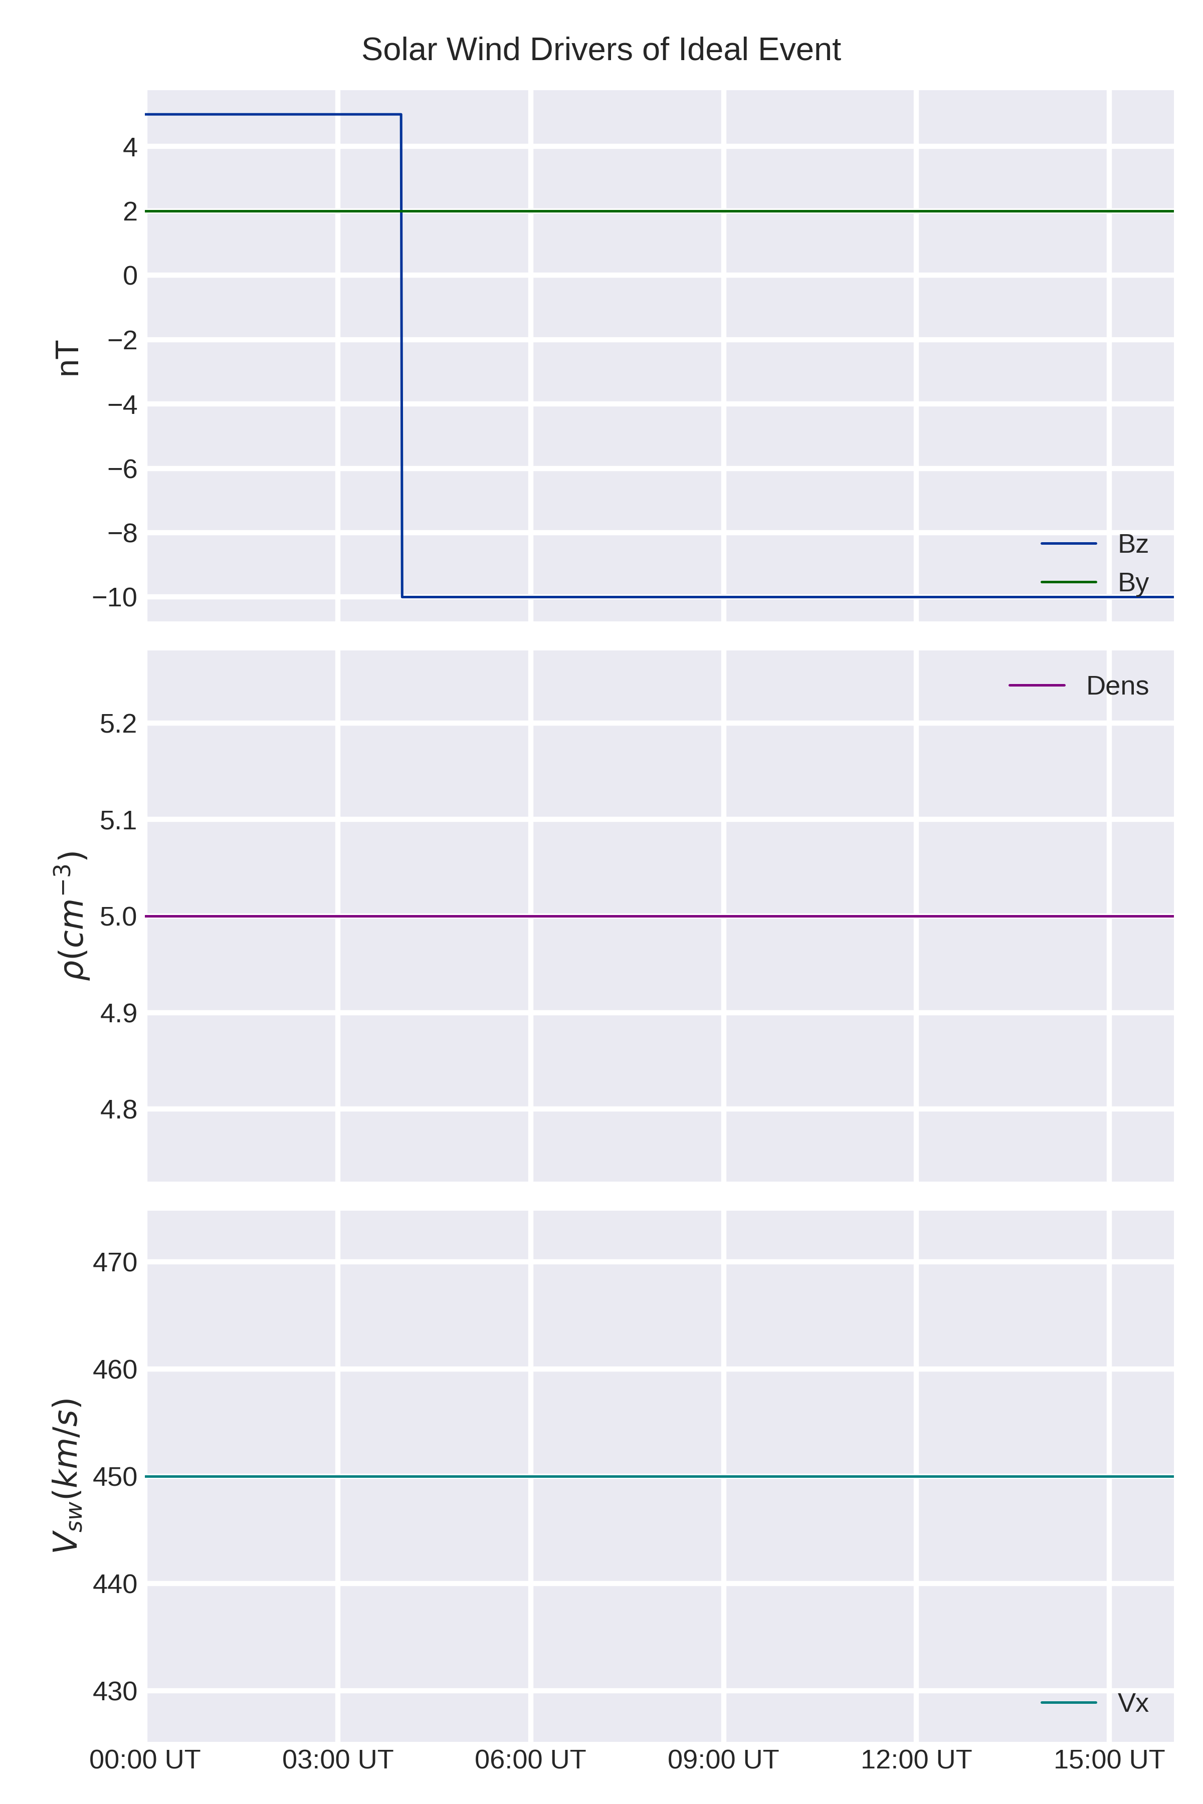
\includegraphics{Ideal_Square_Wave.png}
\caption{IMF conditions of Ideal Square Wave Event.}
\label{fig:1}
\end{center}
\end{figure}

The z-component of the IMF began as a slightly northward +5 nT. After 8 hours of time accurate simulation the z-component turned instantaneously southward to -10 nT. The y-component had a slightly northward +2 nT tilt, removing the day side reconnection line out of the equatorial plane, while the x-component was a constant 0 nT throughout. The velocity of the solar wind was a constant 450 km/s for the entire simulation. The density of the hydrogen was 8.699 particles per cubic centimeter ($/{cm^{3}}$). Due to the aforementioned requirement of the upstream boundary condition a constant density .001 (/$cm^{3}$) was enforced for the plasmasphere fluid. 
\section{A Section Explaining What Katus did in her 2014 paper.}
\section{Time-Epoch Averaged Co-rotating Interaction Region Event}

\begin{figure}[!ht]
\begin{center}
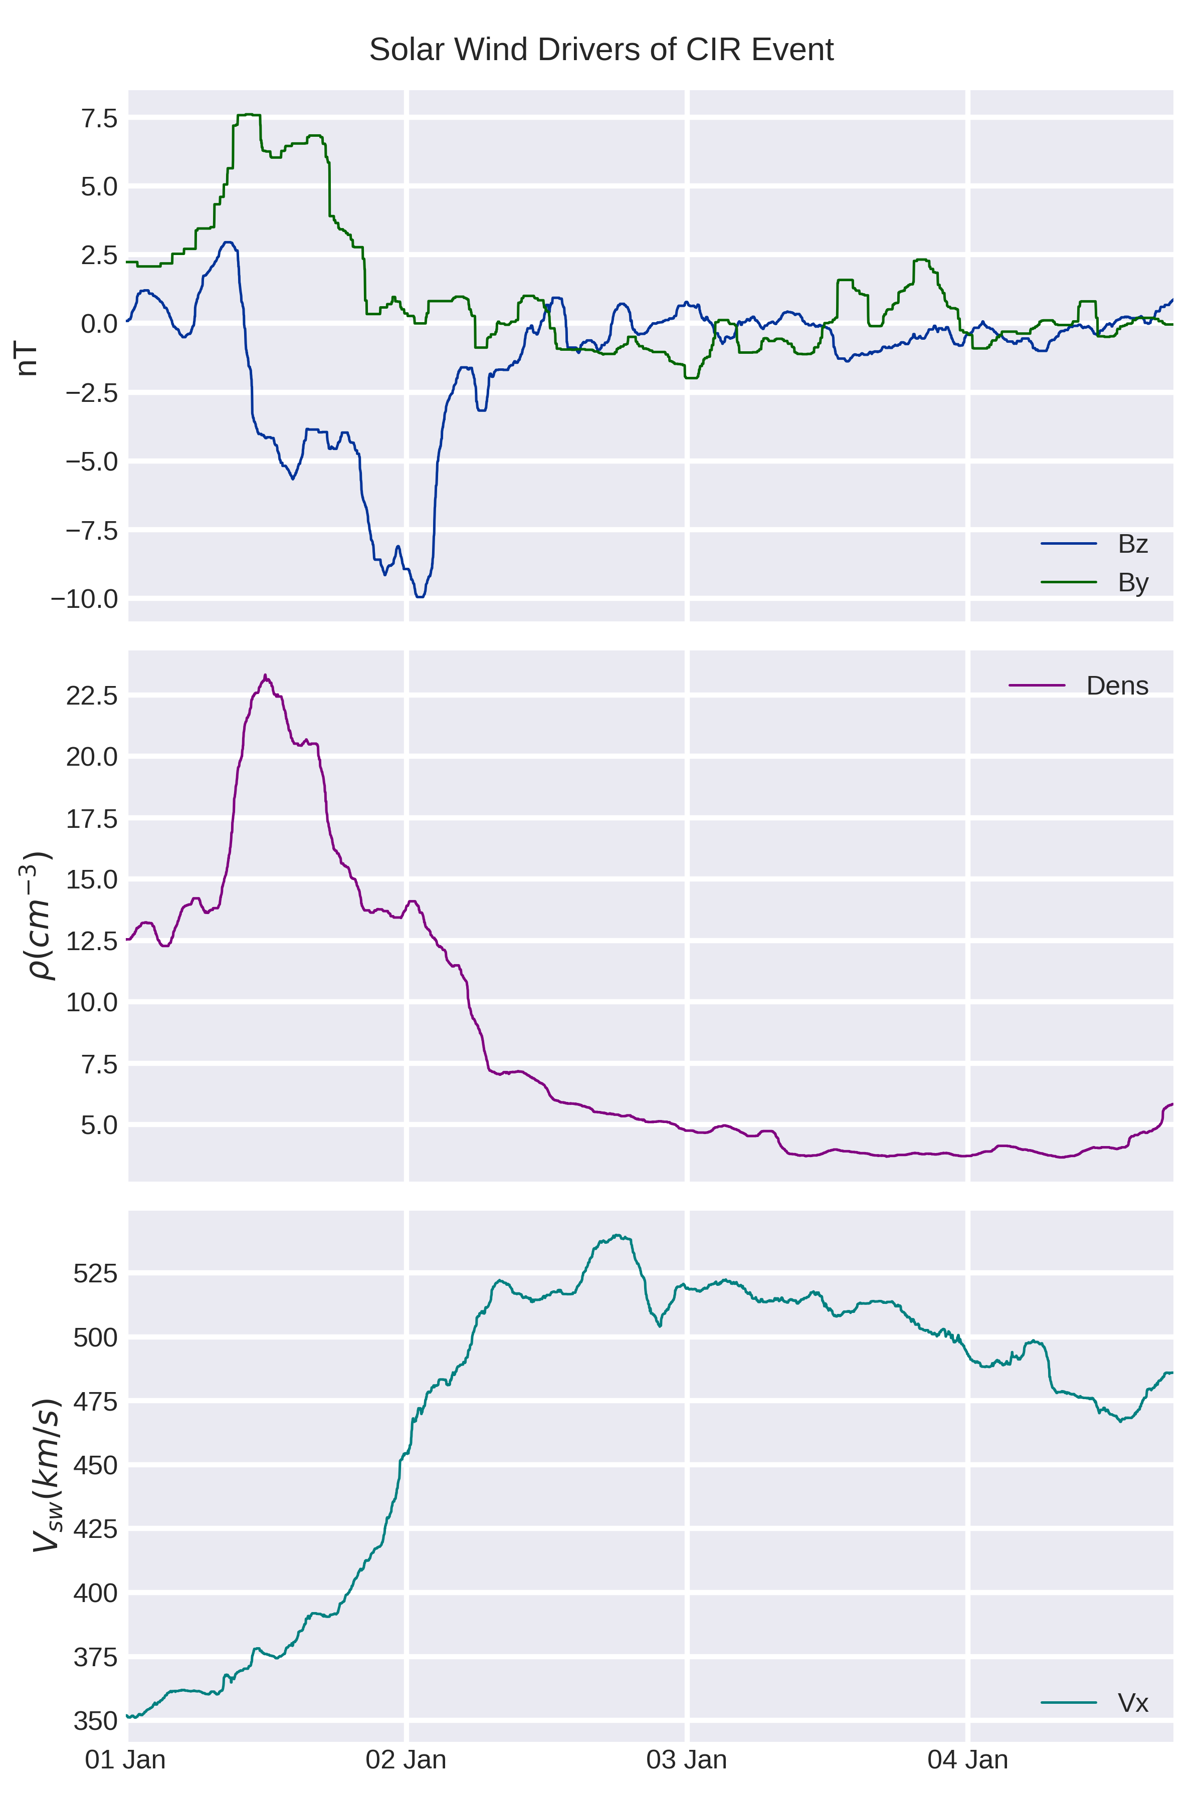
\includegraphics{Ideal_CIR.png} 
\caption{IMF conditions of Corotating Interaction Region Event.}
\label{fig:2}
\end{center}
\end{figure}

\section{Time-Epoch Averaged Coronal Mass Ejection - Magnetic Cloud Event}

\begin{figure}[!ht]
\begin{center}
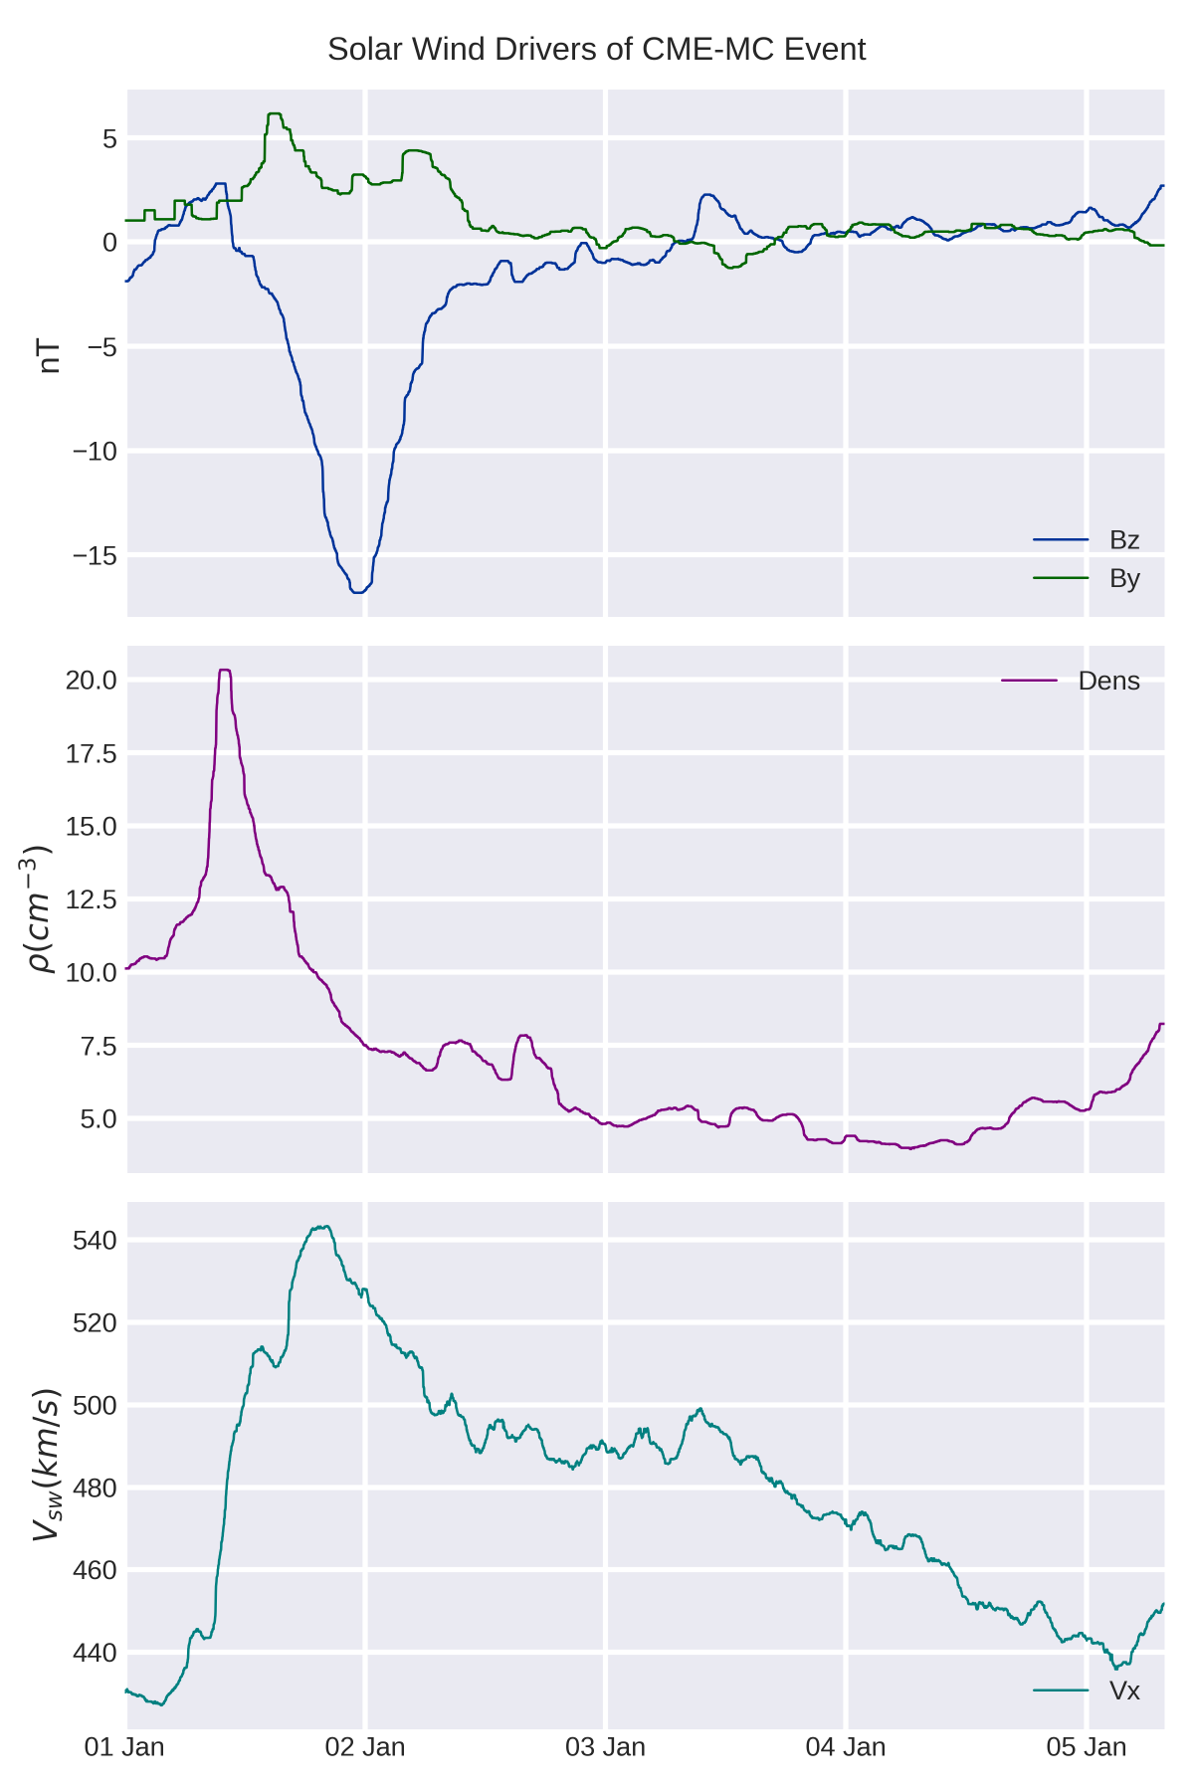
\includegraphics{Ideal Magnetic Cloud.png}
\caption{IMF conditions of Coronal Mass Ejection Magnetic Cloud.}
\label{fig:3}
\end{center}
\end{figure}

\section{Time-Epoch Averaged Coronal Mass Ejection - Sheath Event}

\begin{figure}[!ht]
\begin{center}
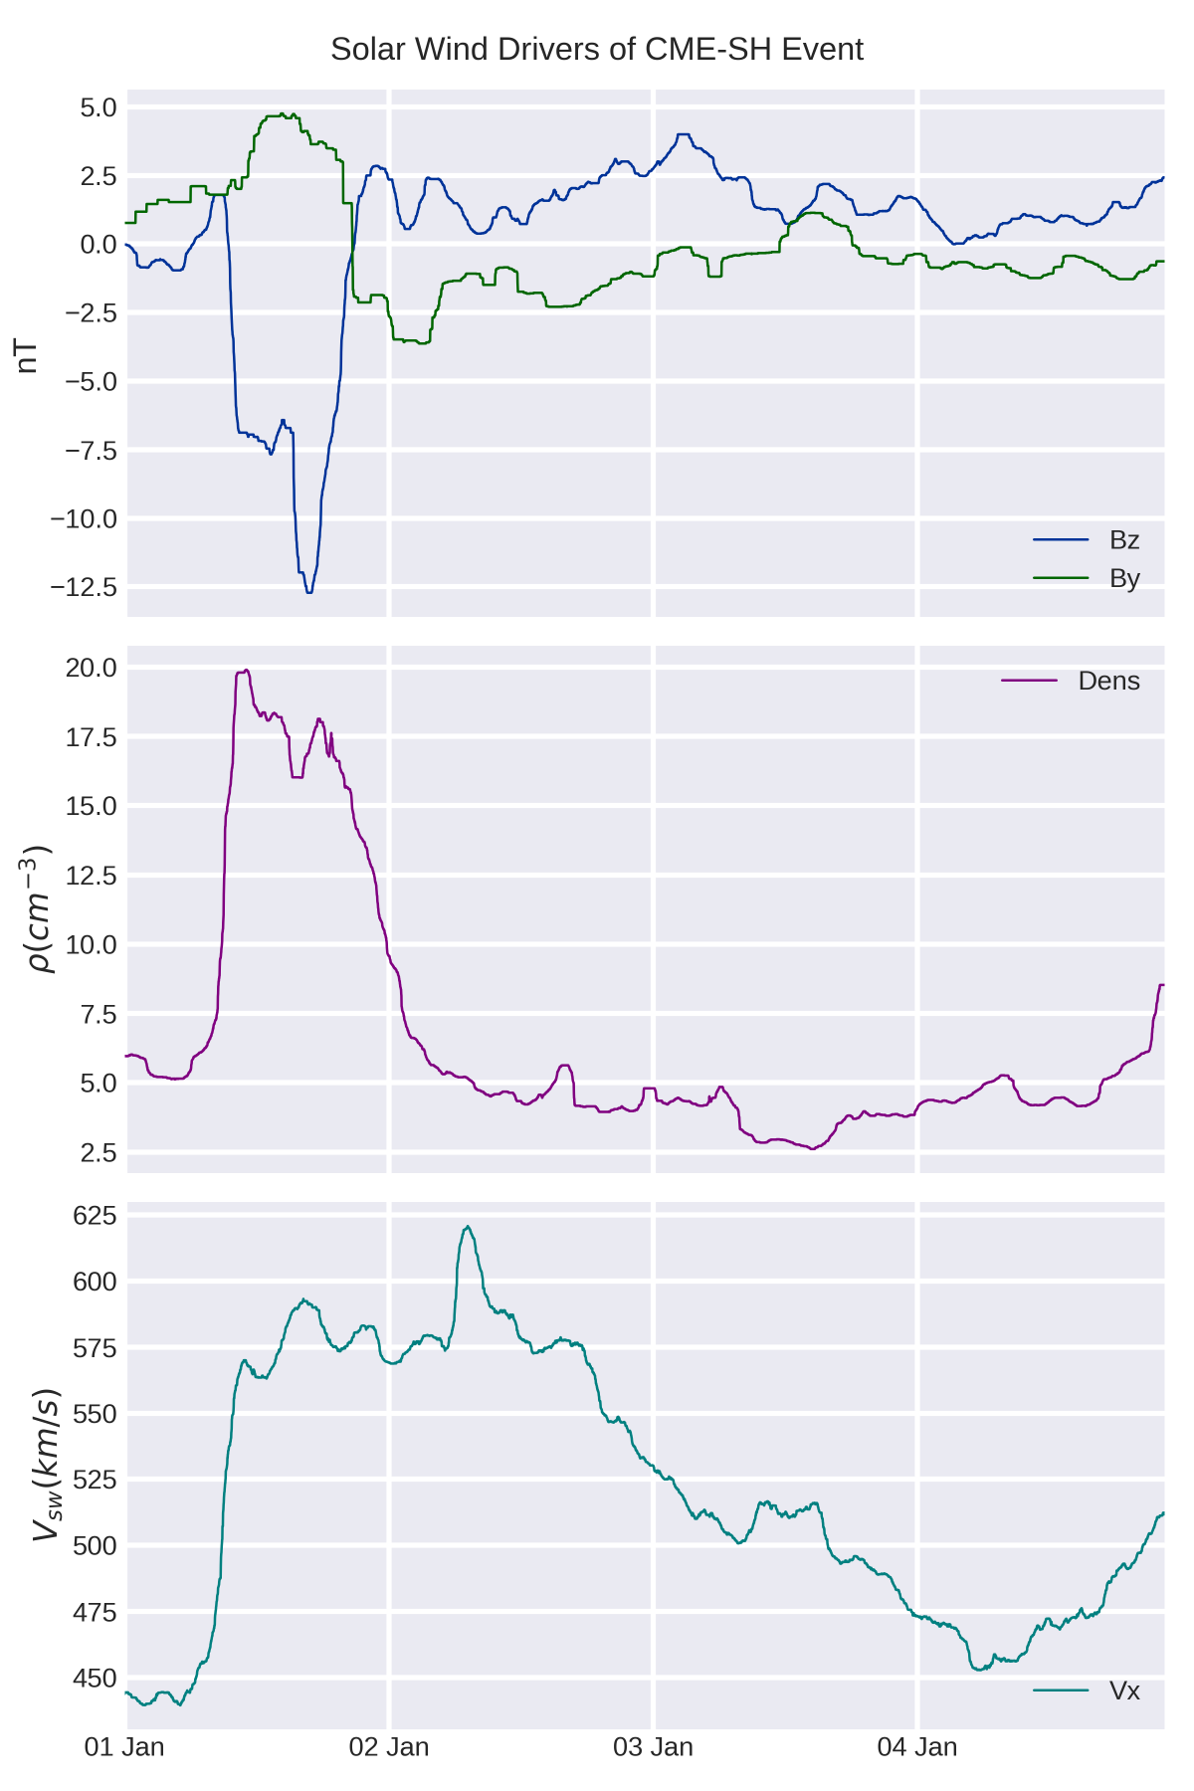
\includegraphics{Ideal_Sheath.png}
\caption{IMF conditions of Coronal Mass Ejection - Sheath Driven.}
\label{fig:4}
\end{center}
\end{figure}

\section{Real World Storm 1}
\section {Real World Storm 2}

\chapter{Analysis}

\chapter{Discussion}

\chapter{Conclusion}
You should let me graduate, 'cuase I did good work that was helpful to the broader space physics community.

\section{Special Thanks}

I would like to thank myself for being the right combination of stubborn and clever to make it through. 
\end{document}